\documentclass[crop]{CSLB}

\usepackage{MySettings}

% #1 is the caption name, #2 is the caption text
\newcommand{\definecaption}[2]{%
   \expandafter\newcommand\csname caption@#1\endcsname{#2}}

\newcommand{\usecaption}[1]{%
   \caption{\csname caption@#1\endcsname\label{#1}}}

% Now the captions

%_______________________________________________________________
\definecaption{F_scheme}{%
%
Space--time diagrams showing a schematic representation of the
different stages in the development of a communicating civilization,
the growing communicating sphere (a) and the temporal intervals for
the communication between two civilizations (b).
%
In the upper panel (a), the sphere the encloses the region which is
causally connected to the emitter grows until it reaches the
$D_{max}$ distance.  After the $D$ event, that region is limited by
the surface of last contact.
%
The scheme in the lower panel (b) represents two communicating
civilizations that have causal contact in both directions
%
}

%_______________________________________________________________
\definecaption{F_messages}{%
%   
Schematic representation of the possible cases in which a
ceti A can be in causal contact with a ceti B which appears later.
%   
The duration of the causal contact in one direction depends on
several factors, mainly $\Delta t_A$, $\Delta t_C$, and $\Delta X$.
%   
}

%_______________________________________________________________
\definecaption{F_number_of_contacts}{%
%
Empirical cumulative distributions of the number contacts
for MPLs in four different samples (M5, M6, M7, M8) with long
range signal reach (D$_{max}$=10000).
%
}


%_______________________________________________________________
\definecaption{F_never_contact}{%
%
Rate of MPLs that never make contact (listening) as a
function of $\tau_a$ and $\tau_s$, for 
$D_{max}$=10000 (left panel),
$D_{max}$=40000 (middle panel), and
$D_{max}$=80000 (right panel)
%
}



%_______________________________________________________________
\definecaption{F_C_at_A}{%
%
Rate of MPLs that listen at the moment of the
awakening, as a funcion of $\tau_a$ and $\tau_s$, for
$D_{max}$=10000 (left panel),
$D_{max}$=40000 (middle panel), and
$D_{max}$=80000 (right panel)
%
} 


%_______________________________________________________________
\definecaption{F_waiting_for_1C}{%
%
Histograms of the mean waiting times for the first contact, for
several models.
%
Left panel shows the histograms for several values of $\tau_a$, and
$\tau_s$ in the range 17000-24000 yr.
%
Right panel shows the histograms for several values of $\tau_s$, and
$\tau_a$ in the range 68000-100000 yr.
%
The shape of the histograms does not change when $\tau_a$ is
modified, but significantly changes when $\tau_s$ is modified.
}
 


%{{{ 
%\begin{figure}
%   \centering
%   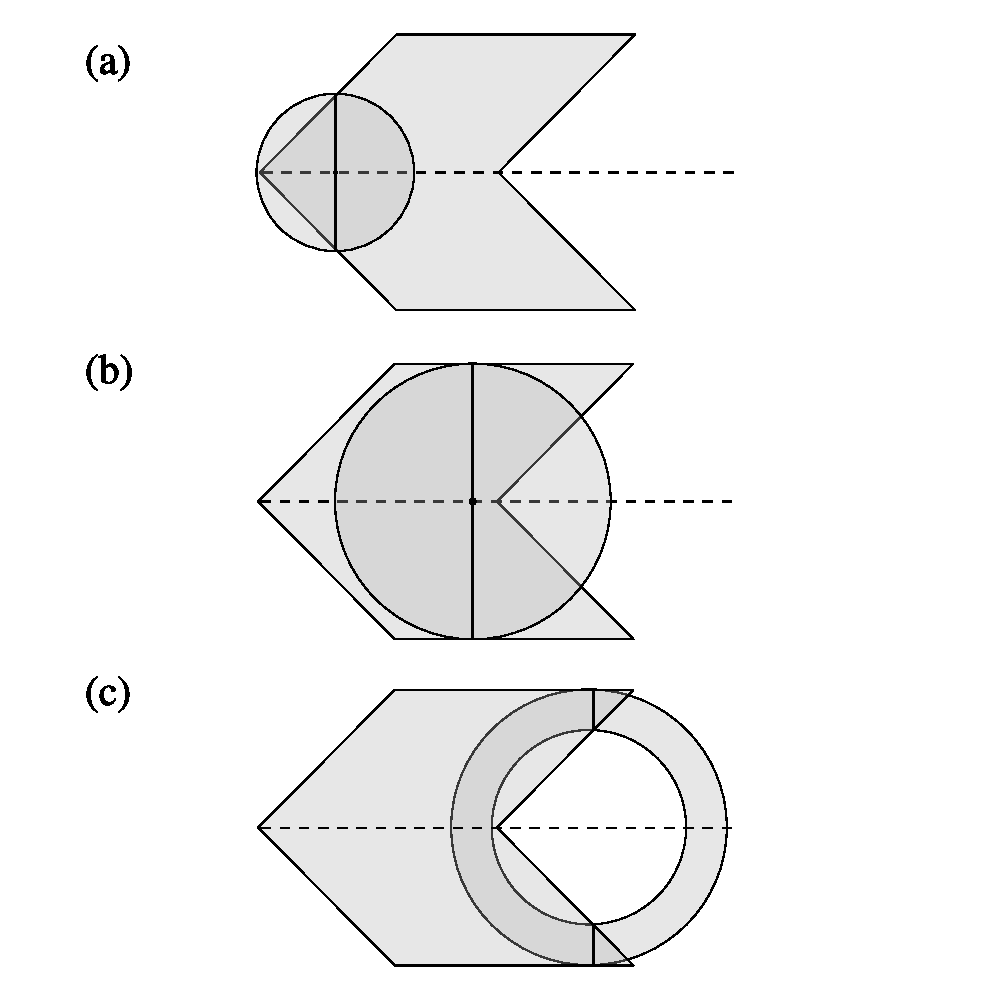
\includegraphics[width=0.5\textwidth]{growingsphere.pdf}
%   \caption{Schematic representation of the growing communicating
%   sphere, over the space--time diagrams, where time is represented on
%   the horizontal direction, and space is represented in the vertical
%   direction.  In (a) the sphere is
%   growing as the surface of first contact has not reached the maximum
%   distance.  In (b) it has reached the maximum distance, so that it
%   remains at the same size.  After a Doomsday event, the signals can
%   still be observed, but the surface of last contact grows }
%   \label{F_growing_sphere}
%\end{figure}
%
%  
%\begin{figure}
%   \centering
%   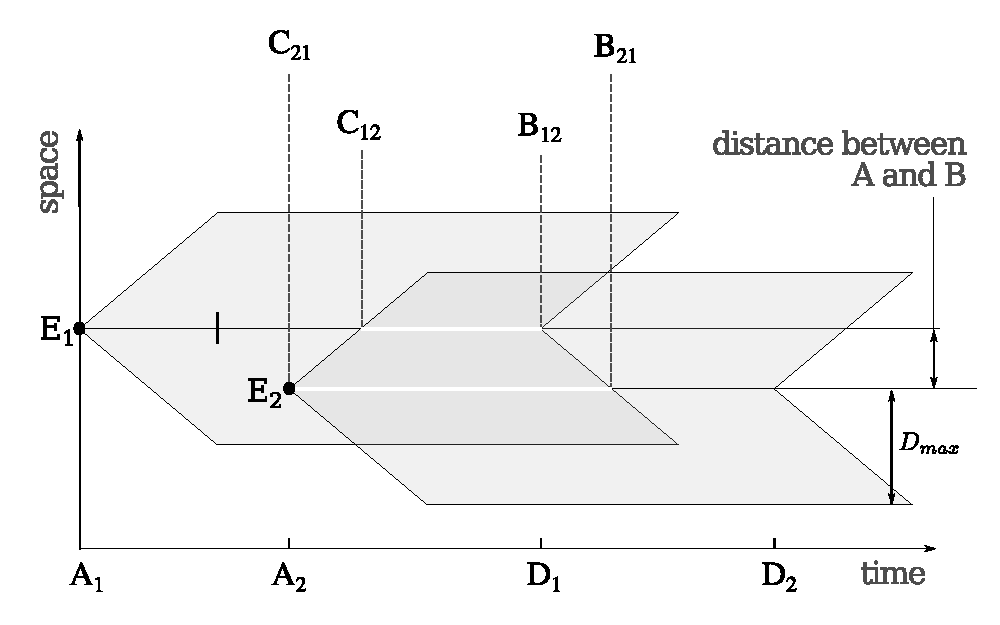
\includegraphics[width=0.5\textwidth]{abcd.pdf}
%   \caption{Schematic representation of two emitters, $E_1$ and $E_2$,
%   that reach each other at different times.  The time span for $E_i$
%   is $(A_i, D_i)$, for $i=\{1,2\}$.  Emitter $i$ can listen to
%   emitter $j$ between $C_{ij}$ and $B_{ij}$.
%   The type and length of causal contact in both directions depend on
%   the distance and time lag between the awakening events, the maximum
%   distance that a signal can reach and the time period in which each
%   emitter is active.}
%   \label{F_abcd}
%\end{figure}

% Schematic representation of the growing communicating
%   sphere, over the space--time diagrams, where time is represented on
%   the horizontal direction, and space is represented in the vertical
%   direction.  In (a) the sphere is
%   growing as the surface of first contact has not reached the maximum
%   distance.  In (b) it has reached the maximum distance, so that it
%   remains at the same size.  After a Doomsday event, the signals can
%   still be observed, but the surface of last contact grows.
%   %
%   Schematic representation of two emitters, $E_1$ and $E_2$,
%   that reach each other at different times.  The time span for $E_i$
%   is $(A_i, D_i)$, for $i=\{1,2\}$.  Emitter $i$ can listen to
%   emitter $j$ between $C_{ij}$ and $B_{ij}$.
%   The type and length of causal contact in both directions depend on
%   the distance and time lag between the awakening events, the maximum
%   distance that a signal can reach and the time period in which each
%   emitter is active.
%
%
%
%   \begin{figure}
%      %
%      \centering
%      %
%      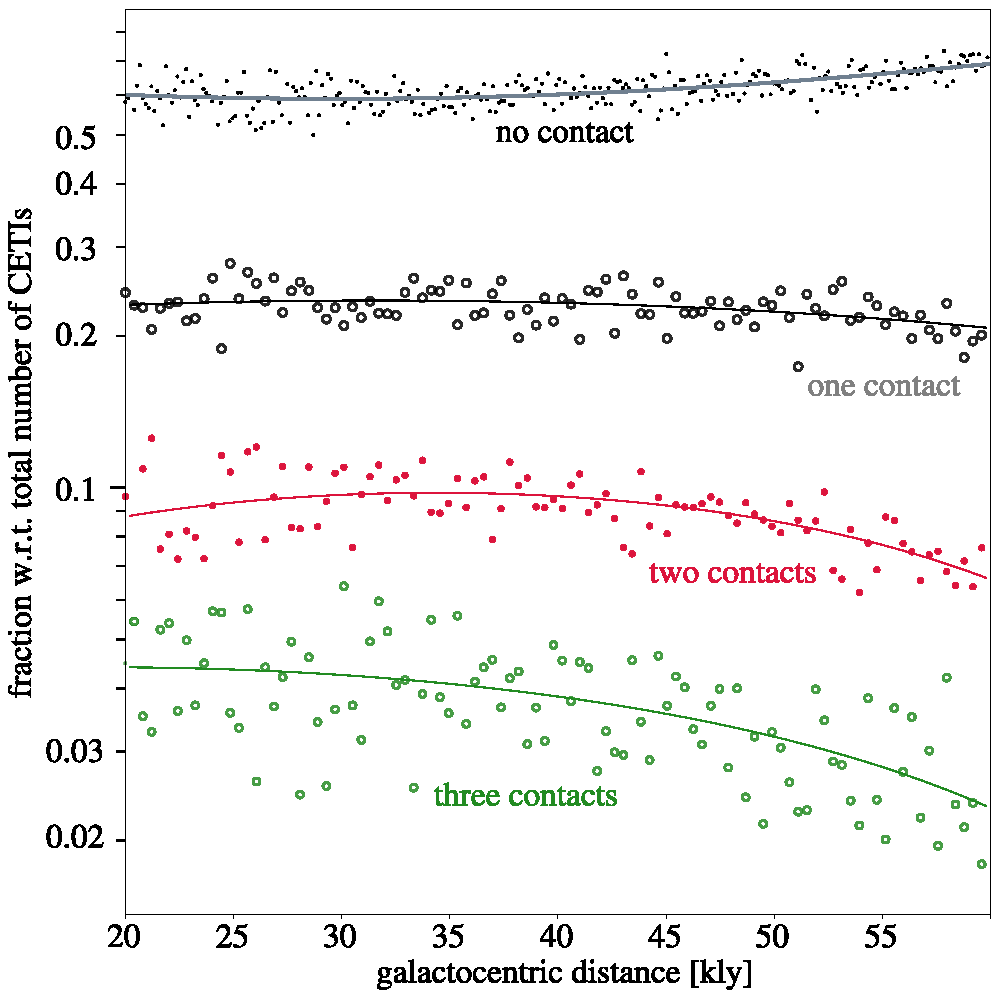
\includegraphics[width=0.45\textwidth]{galactocentric_frac.pdf}
%      %
%      \caption{Fraction of MPLs making cero, one, two or three contacts
%      as a function of galactocentric distance.}
%      %
%      \label{F_radial_frac}
%      %
%   \end{figure}
%}}} 




\begin{document}

\supertitle{Research Paper}

\title[Probabilities of SETI contacts]{Probability of causal
contact between interstellar civilizations through MonteCarlo simulations}

\author[Lares, Funes \& Gramajo]{Lares M.$^{1, 2}$, Funes J.~G.$^{1,
3}$ \& Gramajo L.$^{1, 2}$}

\corres{\name{Lares M} \email{marcelo.lares@unc.edu.ar}}

\address{
   \add{1}{CONICET, Argentina}

   \add{2}{Universidad Nacional de C\'ordoba, Observatorio
           Astron\'omico de C\'ordoba, Argentina}

   \add{3}{Universidad Cat\'olica de C\'ordoba, Argentina}
}
 

\keywords{SETI, Computer simulations, Statistics}

%\JELclassification{XX; XX}
%\MSCcodes{XX; XX}

\Abbreviations{SETI: Search for Extraterrestrial Intelligence,\\
CCN: causally connected node,\\
SFC: surface of first contact,\\
SLC: surface of last contact,\\
DE: Discrete Event,\\
GHZ: Galactic Habitable Zone}
 

\begin{abstract}
%
The abundance of intelligent civilizations in the galaxy is a
longstanding question, which is often conceptualized as the problem
of the lack of received communication or the Fermi paradox.
%
Most efforts on the estimation of a number of intelligent
civilizations are centered on the Drake equation, although 
its factors are affected by large uncertainties, and it lacks a
temporal nature.
%
A alternative approach uses detailed numerical simulations of the galaxy
and recipes for the rates of the formation of stars and planets, and
even for the origin of life.
%
Here we present numerical simulations of stochastic processes of
emergence of civilizations with communication capabilities, based
on minimal asumptions, and analyze the causal connections among them.
%
The analysis of the rate of causal contacts as a function of the mean
number of civilizations, the mean lifetime span distribution and the
maximum distance a civilization can send signals is presented, and
used as a framework to discuss the spatial and temporal structure
of a populated galaxy within several different scenarios.
%
Our results indicate that, given the large distances involved, causal
contacts between civilizations are very rare.
%
Additionally, the odds to make a contact in a few years of monitoring, 
assuming a perfect detection rate, are low for most models, with the
exception of models which propose a galaxy densely populated with
long lived civilizations.
%
The probability of causal contacts increases with the 
mean lifetime of civilizations much more signifficantly than with
the mean number of active civilizations for a given
time window.
%
\end{abstract}

\maketitle


%%% S E C T I O N - - - - - - - - - - - - - - - - - - - - - - -
%%% S E C T I O N - - - - - - - - - - - - - - - - - - - - - - -
\section{Motivations}\label{S_motivations}
%{{{

The Drake equation \citep{drake_intelligent_1962}
offers a very helpful educated guess,
a rational set of lenses --the factors in the equation-- through which
to look at future contacts with a technologically advanced
civilization in the Milky Way.
%
The equation quantifies the number of
civilizations from whom we might receive an electromagnetic signal.
%
A comprehensive review and analysis of each term of the equation
is presented in \citet{vakoch_drake_2015}.
%
\citet{prantzos_joint_2013}
proposes a unified framework
for a joint analysis of the Drake equation and the Fermi paradox
concluding that for sufficiently long-lived civilizations,
colonization of the Galaxy is the only reasonable option to gain
knowledge about other life forms.
%
\citet{haqq-misra_drake_2017}
discuss the dependence of the Drake equation parameters on the
spectral type of the host star and the time since the galaxy formed
and examine trajectories for the emergence of communicative
civilizations over the history of the galaxy.
%
The abundance of
intelligent civilizations in the galaxy is a longstanding question,
which is often conceptualized as the problem of the lack of received
communication or the Fermi paradox 
\citep{barlow_galactic_2012, Sotos_biotechnology_2019,
forgan_galactic_2016}.



There are many proposals aimed at solving this paradox, which make use
of statistical \citep{solomonides_probabilistic_2016,
vanhouten_isthere_2017, horvat_calculating_2007,
maccone_statistical_2015} or stochastic approaches
\citep{forgan_numerical_2009, bloetscher_using_2019,
glade_stochastic_2011, forgan_numerical_2010}, analytical
interpretations of the Drake equation \citep{prantzos_joint_2013,
smith_broadcasting_2009} or more speculative proposals
\citep{barlow_galactic_2013, lampton_information_2013,
conway_three_2018, forgan_galactic_2017}.
%
%%%%% agregar Carroll-Nellenback, 2019).
\Fpagebreak
%
The Drake equation is a key tool
to organize the discussion around the problem of the abundance
of civilizations 
in the Galaxy \citep{hinkel_interdisciplinary_2019}.
%
However, the uncertainties in the factors of this equation make
it less prone to a formal application in order to define searching
strategies or to compute the actual number of extraterrestrial
intelligences.
%
The optimistic estimation from the Drake equation contrast with
the 
SETI initiatives,
noticeable overshadowed by the fact that despite decades of effort, not a
single extraterrestrial intelligence, if any, has been detected.



Some modifications to the original idea of the equation have tried to
imprint a stochastic nature, or to propose a probabilistic approach,
or to consider the temporal structure which is missing in the
equation.
%
Temporal aspects of the distribution of communicating civilizations
and their contacts have also been explored by several authors
\citep{fogg_temporal_1987, forgan_spatiotemporal_2011,
balbi_impact_2018, balb_spatiotemporal_2018, horvat_impact_2011},
%The Impact of the Temporal Distribution of Communicating
%Civilizations on Their Detectability Temporal dispersion of the
%emergence of intelligence: an inter-arrival time analysis The
%spatiotemporal aspects of SETI
%
as well as efforts on considering the stochastic nature of the Drake
equation \citep{glade_stochastic_2011}.
%
The simulation approach has also been considered
\citep{forgan_evaluating_2015, vukotic_grandeur_2016,
murante_simulating_2015, forgan_numerical_2009, forgan_galactic_2017},
although with a similar problem that consists on the large number of
parameters which are either unknown or largely uncertain.
%
%New numerical determination of habitability in the Galaxy: the SETI
%connection
%
%Since the factors in the Drake equation are uncertain,
%
In this work, we propose to avoid the frequentist approach of the
Drake equation and to explore a parameter space, where instead of
computing a final number, we provide a statistical distribution that
gives conditional probabilities.
%
This is an exploratory analysis that aims at providing a numerical
tool to discuss not the several theoretical problems summarized by the
Drake equation factors, but the different scenarios on the basis of
statistical heuristics.
%
The approach proposed here should be considered as a compromise between
the uncertainties of the frequentist approach and the detailed recipes
required on the simulation approach.
%
We then provide a numerical framework to explore via simulations a
parameter space of unknown observables in order to discuss different
scenarios and their consequences in terms of the probability con
making contacts.
%
The only fact that can be stated with certainty is that for the number
of years SETI projects have been working we have not received any
signal, at least within the technical possibilities and the conditions
established by SETI \citep{tarter_search_2001}.
%
This arguably astonishing result has lead to the Fermi paradox, which
states an apparent contradiction between the high estimation of the
abundance of life in the Galaxy and the lack of their detection
\citep{vanhouten_isthere_2017}.
%
The lack of detection has also inspired to a number of alternative
proposals for new SETI strategies \citep{forgan_exoplanet_2017,
balbi_impact_2018, loeb_eavesdropping_2006, maccone_KLT_2010,
tarter_advancing_2009, enriquez_breakthrough_2017, loeb_relative_2016,
maccone_SETI_2011,  lingam_relative_2019, wright_theGsearch_2015,
maccone_SETI_2013, maccone_lognormals_2014, harp_application_2018,
forgan_possibility_2013, forgan_galactic_2017, funes_searching_2019}.
 


The discrete events method for simulating a stochastic process is an
approximation that allows to study the behavior of complex systems,
by considering a sequence of well defined discrete events.
%
The simulation is carried out by following all the variables that
describe and constitute the state of the system, and the evolution of
the process is described as a set of changes in that state.
%
In this context, an event produces a specific change in the state,
that can be triggered by random variables that encode the stochastic
nature of the physical phenomenon.
%
For example, when a new contact is produced between two entities in
the simulated galaxy, the numbers of active communication lines and of
active communicated nodes change.
%
The process involves then following the changes on the state of the
system, defining the initial and final states, defining a method that
allows to keep track of the time progress in steps, and maintaining a
list of relevant events.


In a recent work, \citep{balbi_impact_2018} use a statistical model to
analyze the occurrence of causal contacts between civilizations in the
Galaxy.
%
The author highlights the effect of evolutionary processes when
attempting to estimate the number of communicating civilizations that
might be in causal contact with an observer located on the Earth.
%
\citet{cirkovic_temporal_2004} also emphasize the lack of temporal
structure in the Drake equation.
%
\citet{bloetscher_using_2019} uses a probabilistic approach, though
still strongly motivated by the Drake equation, to obtain a
probabilistic measure for the number of civilizations in the Galaxy.
%
To that end, perform MonteCarlo Markov Chains over each factor of the
Drake equation, and combine the means to obtain a probabilistic
result.
%
It is worth mentioning that the author proposes a log-normal target
distribution to compute the posterior probabilities.
%
This approach, which assigns probability distributions to the Drake
factors.
%
This study concludes that there is a very low probability for Earth to
make contact with another extraterrestrial civilization.    
%
\citet{smith_broadcasting_2009} uses a analytical model to compute the
probabilities of contact between two randomly located civilizations,
and the waiting time for the first contact, assuming a fixed maximum
broadcasting distance.
% 
\citet{balbi_impact_2018} investigate the chance of communicating
civilizations making causal contact within a volume surrounding the
location of the Earth, using a statistical model to compute the
occurrence of causal contacts. The author stresses the fact that the
causal contact requirement involves the distance between
civilizations, their lifespan and their times of appearance.  This is
important since the time it takes the light to travel across the
Galaxy is much lesser than its lifetime.
%
\citet{balbi_impact_2018} fix the total number of civilizations and
explore the parameter space that comprise three parameters, namely,
the distance to the Earth, the time of appearance and the lifespan of
the communicating civilization.
%
Each of these three variables are drawn from a random distribution.
The distribution of the distances results from a uniform distribution
of civilization within the plane of the Galaxy.
%
For the distribution of the characteristic time of appearance, the
author explores and exponential and a truncated Gaussian
distributions. For the distribution of the lifespans, the author
chooses an exponential distribution.
%
The radius of influence is set to 1000 lyr.
%
\citet{balbi_impact_2018} finds that the fraction of communicating
civilizations vary with the choice of the statistical distribution for
the time of appearance. For all analyzed distributions, the fraction
corresponding to a mean lifetime of 10$^9$ years and for a maximum
radius for the detection of the signal of 1000 yr, is roughly 0.1.
%
\citet{vukotic_astrobiological_2012} propose a simulation approach
based on probabilistic cellular automata (PCA) modeling. In this
framework, a complex system is modeled by a lattice of cells which
evolve at discrete time steps, according to transition rules that take
into account for each cell the states of its neighbor cells.
%
The authors implement a PCA model to a network of cells which
represent life complexity on a 2-dimensional annular ring resembling
the GHZ. The authors set the GHZ between a minimum radius of 6 kpc and
a maximum radius of 10 kpc. Within this framework, the authors also
make several MonteCarlo simulations and analyze ensemble-averaged
results.
%
This work aims at analyzing the evolution of life, although it does
not account for the network of causal contacts among technological
civilizations.


In this work we address the problem of the temporal and spatial
structure of the distribution of communicating civilizations, by
exploring the hypothesis space over a minimal set of parameters.
%
In Sec.~\ref{S_methods} we introduce the methods and discuss the
candidate distributions for the statistical aspects of the times
involved in the communication process.
%
Then, we present our results in Sec~\ref{S_results}, with special
emphasis on the statistical distributions of the duration of causal
contacts in one or both directions, the possible differences on the
position of a civilization on the Galaxy and the distribution of time
intervals for the waiting of the first contact, always as a function
of the three simulation parameters.
%
Finally, in Sec.~\ref{S_discussion} we discuss our results and future
research directions.


% HACER DISCUSION FUERTE DE ESTOS PAPERS: \cite{balbi_impact_2018,cirkovic_temporal_2004,grimaldi_signal_2017,smith_broadcasting_2009}

%}}}



%%% S E C T I O N - - - - - - - - - - - - - - - - - - - - - - -

\begin{figure}
   \centering
   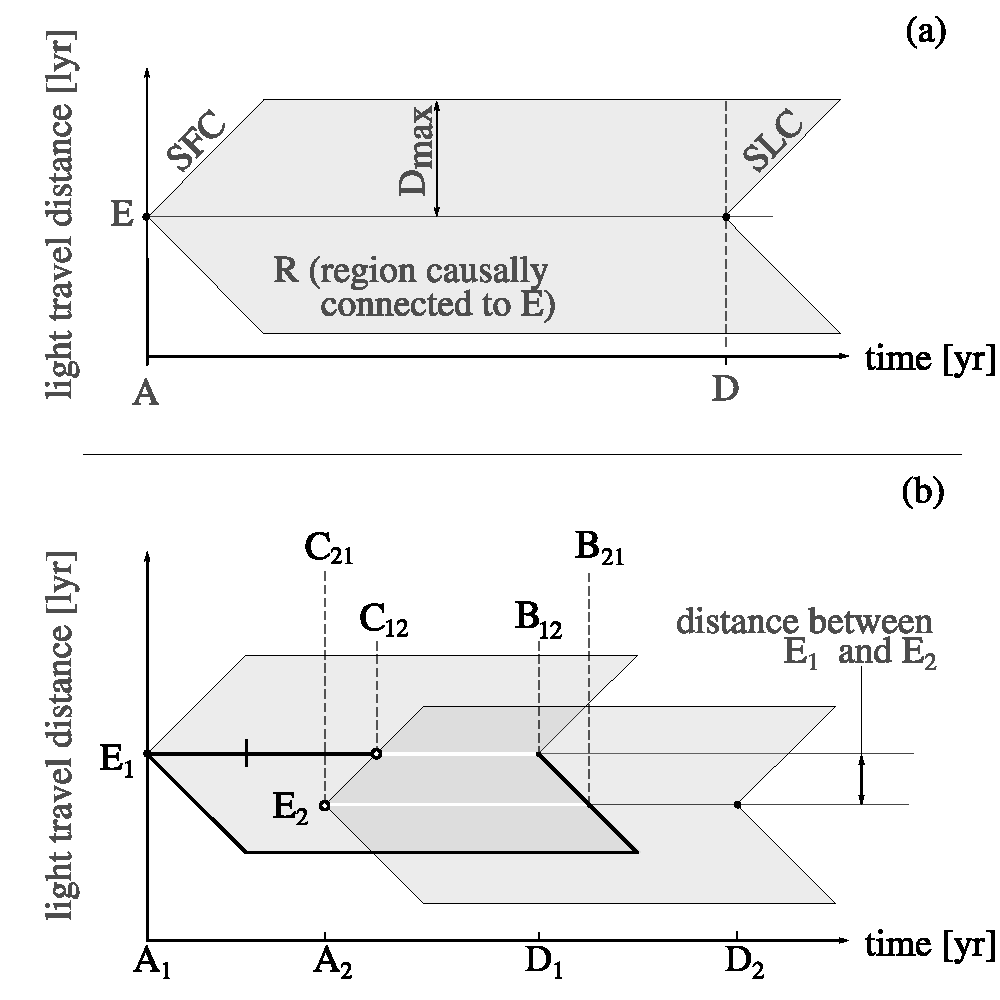
\includegraphics[width=0.5\textwidth]{F_scheme.pdf}
   \usecaption{F_scheme} \label{F_scheme}
\end{figure}
 
\begin{figure*}
   \centering
   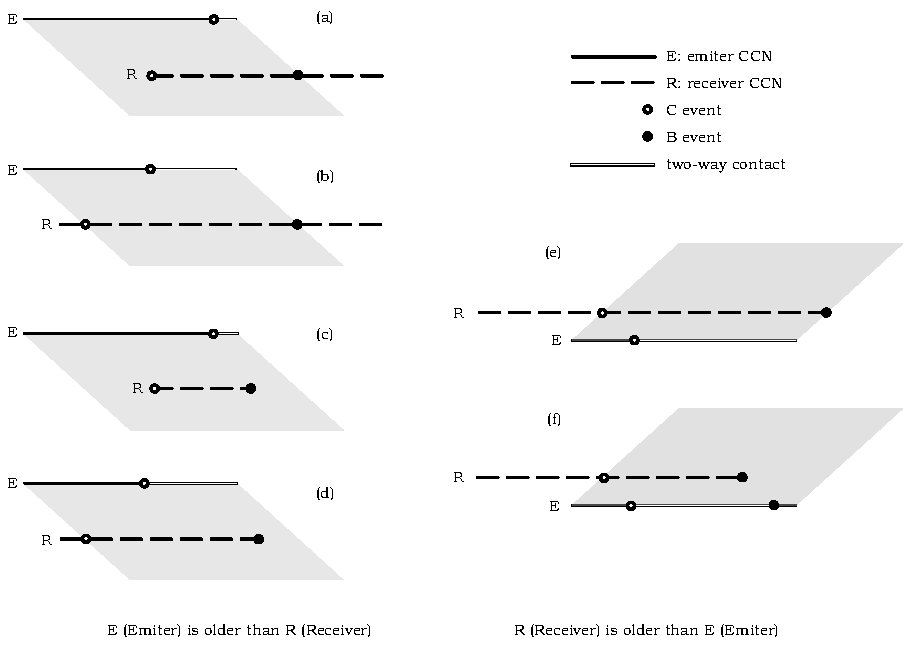
\includegraphics[width=0.8\textwidth]{F_messages.pdf}
   \usecaption{F_messages} \label{F_messages}
\end{figure*}
      

%%% S E C T I O N - - - - - - - - - - - - - - - - - - - - - - -
\section{Methods and working hypotheses}\label{S_methods}
%{{{

Simulations are suitable tools to analyze systems that evolve with
time and involve randomness.
%
An advantage of simulations compared to theoretical approaches, is
that the former usually require less assumptions and simplifications,
and can be applied to systems where a theoretical model can not be
found.
%
In particular, many complex stochastic processes that can be described
by the evolution of the state of a system, can be efficiently modeled
with the discrete--event (hereafter, DE) simulation approach.
%
A system described with the DE paradigm is characterized by a set of
actors and events, where actors interact causally through a series of
events on a timeline and process these events in chronological order
\citep{ptolemaeus_system_2014, chung_simulation_2003,
ross_simulation_2012}.
%
Each event produces changes in the values of the variables that define
the process, and thus the corresponding change in the state of the
simulated system.
%
This method is well suited for the particular case of the diffusion of
intelligent signals in the Galaxy, and allows to explore several
models easily.
%
We simulate the statistical properties of a set of points in space and
time that have a causal connection
at light speed, hereafter dubbed ''causal contact nodes'' (\ceti).
%
% ability of emitting and receiving messages at
%
We chose this generic name in order to stress the fact that in this
analysis no broadcasting or lookout activities are required, 
and therefore not actual messages are considered, only the causal
contact.
%
For the special case of a fully efficient node that emits
and receives isotropically, a causal contact node can be considered as
a broadcasting station that has the ability to detect signals through
an active lookout program.
%
Also, it is worth mentioning that this is a general approach, and not
necessarily a \ceti is the host of an intelligent civilization.
%
It can be associated with a planet where life has developed,
became intelligent, reached the skills required to find the right
communication channel, sustain a search and establish a contact.
%
Alternative message processing entities could be considered, for
example interstellar beacons where life has ceased to exist but
continue with its emission or communication stations established by
probes or left intentionally by intelligent beings \citep[see, e.g.,
][]{peters_outer_2018, barlow_galactic_2013}.
%
In principle, these strategies could affect our results since it would
be easier to configure a cluster of \cetis that spread in time.
%
However, we do not consider this highly speculative alternatives at
this point.
%
% have been proposed
%
For the purpose of this analysis, only the communication capability is
relevant, since we study the causal contacts between the locations.
%
The system is defined by a number of actors that represent \cetis and
appear at different instants in time, generating events that produce
meaningful changes in the variables that describe the system, i.e., in
the arrangement of \cetis and their network of causal contacts.
%
For example, the appearance of a new \ceti in a region which is filled
with a signal emitted by another \ceti, will increase the number of
active \cetis and the number of pairs of \cetis in causal contact.
%
Assuming some simple hypotheses, the discrete events method can be
performed taking into account a small number of variables, which allow
to analyze the variation of the results in the model parameter space.


In what follows, we describe the experimental setup chosen to estimate
the probabilities of causal contacts and several derived quantities in
terms of three independent parameters, namely, the mean time span
between the appeareance of consecutive \cetis, ($<\tau_a>$), their mean
lifetime ($<\tau_s>$), and the maximum distance a signal can be
detected by another \ceti ($D_{max}$).
%
Intuitively, the shorter the $\tau_a$ parameter and the larger the
$\tau_s$ and $D_{max}$ parameters are, the greater the probability of
the existence of causal contacts between pairs of \cetis would be.
%
We also need to propose theoretical distribution functions for both
the distribution of lifespans ($\tau_s$) and the distribution of the
number of \cetis per unit time \citep{maccone_evolution_2014,
Sotos_biotechnology_2019}, related to the time span between the
appeareance of consecutive \cetis (since when $<\tau_a>$ is shorter, it
produces a greater density of \cetis).
%
The shapes of these distributions are set to a fixed law, as discussed
in Sec.~\ref{SS_PDF_shape}.


A causal connection can be produced without the need of the two
involved locations being concurrent or active at the same time.
%
This is a fundamental property of the system which arises as a
consequence of the large spatial and temporal scales, where a message
is transmitted at light speed.
%
Although a \ceti could be active for enough time so as to transmit a
message at large distances, the limited power of the message and the
dilution that runs as the squared distance from the source, imposes a
detectability limit.
%
As a consecuence of this limitation and of their finite lifetime,
considered as the period of time between the acquisition and loss of
communicating capacity, each \ceti will fill a spherical shell region of
the Galaxy, limited by two concentric spherical surfaces.
%
The leading front, or surface of first contact (SFC) grows from the
central \ceti until it reaches the maximum distance $D_{max}$.
%
Thus, the volume reached causally by a \ceti is initially a growing
sphere.
%
Following the end of the civilization, there is still a region which
is filled with the emitted signals.
%
The trailing front, or surface of last contact (SLC) also grows from
the central \ceti, with a delay with respect to the SFC equivalent to
the lifetime of the \ceti, and produces a spherical shell region.
%
Any other \ceti within this region will be aware of the originating
\ceti,
even if it has disappeared before the time of contact.
%
This region will grow if the surface of first contact has not yet
reached the maximum distance $D_{max}$, and will shrink otherwise
until the surface of last contact reaches $D_{max}$, producing as a
result the loss of all signal from the central \ceti.
%
In our approach, we consider a model Galaxy where the width of the
disk is negligible with respect to the radius of the disk, so that the
\cetis are placed on a 2D plane disk.
%
In the 2D simulation only the intersection of the communicating
spherical shells with the plane of the galaxy is relevant, and produce
the corresponding circles or rings for the filled spheres or annular
regions of the spherical shells, respectively.
%
We illustrate in the Fig.~\ref{F_scheme} the schematic representation
of the region causally connected to the central \ceti.
%
To this end, we use space--time diagrams, where time is represented on
the horizontal axis, and space is represented in the vertical axis.
%
A growing surface of first contact in this diagram is represented as a
growing circle, centered on a point in the time axis, which shifts
towards the right at the same rate the radius of the circle increases.
%
The maximum distance of the message limits the radius of the circles,
so that once this distance is reached, the circle continues its shift
towards the right, but maintaining a constant radius.
%
At the end of the lifetime of a \ceti, a growing surface of last
contact is represented by a circle that covers the inner part of the
causal region, producing a ring of diminishing area (panel (a)).
%
In this scheme, the entire lifetime of a \ceti can then be represented
by a polygon, limited in the spatial axis by the maximum distance of
the signal $D_{max}$ and in the time axis by the time span between the
starting time (concave vertex) and the ending time (convex vertex).
%
This representation allows to easily visualize the important events
that result from the existence and communications of two \cetis (panel
(b)).
%
The points in time where the \cetis acquire their communicating capacity
(CC) are dubbed ''awakening'' events ($A_1$ and $A_2$ in the Figure).
%
Similarly, the points in time where the \cetis loss their
communicating capacity are dubbed ''doomsday'' events ($D_1$ and $D_2$
in the Figure).
%
The points in space--time where the first contact is produced for each
one of the \cetis, are defined as ''contact'' events, shown as $C_1$
and $C_2$ in the Figure.
%
Finally, the two points where the contact is lost for each one the
\cetis, are denominated ''blackout'' events, shown as $B_1$ and $B_2$
in the Figure.
%
It is important to notice that there is a time delay between the
contact events of the two \cetis involved in this analysis, and also a
time delay between the two blackout events, so that the time range
when a bidirectional contact is possible occurs between the maximum
time of the contact points and the minimum time between the blackout
points.




The initially growing communicating sphere, is shown over
space--time diagrams, where time is represented on the horizontal
direction, and space is represented in the vertical direction.
%
In the upper panel (a), the sphere is growing as the surface of first
contact has not reached the maximum distance.
%
In the middle panel (b) it has reached the maximum distance, so that
it remains at the same size.
%
After a Doomsday event (bottom panel, b), the signals can still be
observed, but the surface of last contact grows.
%
We also show in this Figure a schematic representation of two
emitters, E$_1$ and E$_2$, that reach each other at different times.
%
The time span for E$_i$ is (A$_i$ , D$_i$) , for $i = {1, 2}$.
%
Emitter $i$ can listen to emitter $j$ between C$_{ij}$ and B$_{ij}$.
%
The type and length of causal contact in both directions depend on the
distance and time lag between the awakening events, the maximum
distance that a signal can reach and the time period in which each
emitter is active.
%
In the Fig.~\ref{F_messages} we show a schematic representation of the
possible cases in which a \ceti E can be in causal contact with a
\ceti
R.
%
The duration of the causal contact in one direction depends on several
factors, mainly the lifetimes, the time period between the A events 
and the distance between the two \cetis involved in the causal
contact.



The temporal structure of the process is defined by two distribution
parameters that represent the mean time interval that an intelligent
civilization can emit and receive signals, and the mean time interval
between the emergence of an intelligent communicating civilization and
the next one.
%
The spatial structure of the simulation is given by the size and shape
of the Galactic Habitable Zone and the maximum distance a signal can
travel to be detected.
%
The parameters for the temporal distributions also determine the
spatial properties since the density of active \cetis in the Galaxy
depend on these two parameters.
%
For example, a small $\tau_a$ and a large $\tau_s$ will produce a
Galaxy densely populated with \cetis, and vice versa.
%
Also, some hypotheses must be made in order to complete the
simulation.
%
\citet{forgan_spatiotemporal_2011} argues that the times at which
different civilizations become intelligent follow a Gaussian
distribution, and then the distribution of inter-arrival times is an
inverse exponential.
%
We chose to assume that the distribution of the times of A events is a
stationary Poisson process, and then the distribution of the times
between the appeareance of new consecutive \cetis is exponential.
%
Regarding the duration of a \ceti, we propose that the distribution of
the duration of \cetis is a stationary exponential distribution.
%
\citet{balbi_impact_2018} stress the fact that it would be desirable
to arrive at a theoretical statistical distribution of the lifespan of
civilizations, preferentially on the basis of the underlying
astrophysical and biological processes.
%
\citet{maccone_lognormals_2014} argues that this distribution should
be a log normal.  (EXPAND)



There is no a temporal window for the model, i.e., the simulation
starts when the process is already stable, and ends before any
galactic effect could modify or affect of fixed variables.
%
The probability for the rise of a \ceti is homogeneous over the GHZ.
%
Although the Galaxy has a well known spiral structure, the assumed
sparsity of civilizations makes this assumption very reasonably.
%
Otherwise, if the distribution of civilizations is not sparse, it
could be the case that the spiral arms would host most of the
civilizations, and contacts are frequent between closely located
civilizations.
%
In such a case we could expect that the interpretation of our results
could be considered as pessimist for the establishment of a contact with
our planet.
%
We also limit the posibilities of life or other types of civilizations
to the hypothesis usually stated for the definition of the GHZ
\citep{dayal_habitability_2016, gonzalez_galactic_2001,
lineweaver_galactic_2004, gonzalez_habitable_2005,
morrison_extending_2015, haqq-misra_evolution_2019,
rahvar_cosmic_2016, gobat_evolution_2016, rahvar_cosmic_2016}.
%
\citet{vukotic_astrobiological_2012} propose probabilistic cellular
automata model to explain the astrobiological history of the Milky
Way.
%
This means that we set aside possible civilizations that could survive
in severe conditions or unstable systems, which would prevent the
appeareance of life as we know it.


While the aforementioned assumptions are basic conditions for most of
the stochastic processes observed in nature, we need to make stronger
assumptions related to the nature of the message.
%
The most simple assumption about the message itself, is that it
travels at light speed.
%
With this, we are considering messages sent through, for example,
electromagnetic radiation or even gravitational radiation, but we set
apart messages sent with mechanical means or physical objects, or
through some unknown technology that violates the known so far laws of
physics.
% 
For the communication of \cetis through messages sent isotropically, we
assume that the capacity to emit signals and to receive signals occur
at the same time.
%
This means that the ability to find another civilization develops at
the same time that the ability and intention to emit a signal in all
direction, intended to be detected by an unknown civilization.
%
Although there are several reasons to think that this could not be the
case, at large time scales it can be considered that both abilities
occur roughly at coincident epochs.
%
Another essential assumption is that all \cetis use the same signal
power, so that there is a maximum distance out to which it can be
detected.
%
It is worth mentioning that we are considering in our experimental
setup a system composed by several emiters and receivers across the
Galaxy, under the hypothesis proposed before.
%
In such a system we compute probabilities of a \ceti making contact
with another \ceti, and the results must be interpreted as for a
randomly chosen \ceti, given certain conditions of homogeneity on an
ensemble of equivalent galaxies.
%
We stress the fact that we are not centered on the probabilities for
the Earth itself, but on a generalized \ceti.
%
Regarding the extent of the signals, we know that the distance from
which a signal from Earth could be detected using the current
technology is of a few hundreds light years, given that the signal was
sent to a specific direction.

               

%https://setiathome.berkeley.edu/forum_thread.php?id=80585&postid=1833000#1833000]
%https://www.engadget.com/2017/05/25/listening-to-starlight-our-ongoing-search-for-alien-intelligenc/]
%[from https://en.wikipedia.org/wiki/Fermi_paradox]
%
It is straightforward to propose and implement a distribution of
maximum distances, although this would increase the model complexity
at the cost of a larger uncertainty or of another dimension on the
hypothesis space.
%
This proposal is based on a pronoid scenario (REF), and we do not
consider in this work the occurrence of paranoid or partially paranoid
civilizations.
%
If that would be the case, the results obtained here can be taken as
upper limits.



In our simulations we also assume the simplest situations for the
growth of the sphere of first contact.
%
For example, we discard the possibility of stellar colonization
\citep[e.g.][]{newman_galactic_1981, walters_interstellar_1980,
starling_virulence_2013, barlow_galactic_2012, jeong_large_2000,
maccone_mathematical_2011} and assume that the communication aim is
performed to all directions with the same power and the same
probability, i.e., strongly assume isotropic communication in all
cases.
%
More detailed simulations could be produced considering different
efficiency of communication or detection methods.
%
%Also, a mixed paranoid/pronoid population of intelligent civilizations
%could be implemented easily.
%
% EXPLICARLO O SACARLO
% O PONER EN LA DISCUSION
%
However, in this case we also would complicate the experimental setup,
make the results less evident.
%
The results are independent of the nature of life (organic or
artificial).
%
The lifetime of a civilization can be caused by auto destruction or by
external factors.
%}}}


\subsection{Power laws vs. exponential laws}\label{SS_PDF_shape}
%{{{

The power law and exponential statistical distributions are among the
most common patterns found in natural phenomena.
%
For example, the distribution of the frequency of words in many
languages is known to follow a Zipf law (which is a power law).
%
Zipf law also describes population ranks of cities in various
countries, corporation sizes, income rankings, ranks of number of
people watching the same TV channel (Zipf's law).
%
% CITAR ALGO DE LA LEY DE ZIPF
%
The magnitudes of earthquakes, hurricanes, volcanic eruptions and
floods; the sizes of meteorites or the losses caused by business
interruptions from accidents, are also well described by power laws
(Sornette 2006).
%
The power law behaviour has been observed in a variety of systems,
including for example stock market fluctuations, sizes of computer
files and word frequency in languages \citep{mitzenmacher_brief_2004,
newman_power_2005, simkin_theory_2006}
%
Power laws have also been widely used in biological sciences, e.g., in
analyzing connectivity patterns in metabolic networks
\citep{jeong_large_2000} and in the number of species observed per
unit area in ecology \citep{martin_origin_2006, frank_common_2009}.
% 
More examples can be found in the literature
\citep{martin_origin_2006, maccone_KLT_2010, barabasi_scale_2009,
maccone_evolution_2014, maccone_lognormals_2014,
benguigui_classificacion_2016}
 


In this work, the exponential distribution of lifespan and waiting
times is justified by considering the hypothesis that the process of
appeareance of life in the galaxy is homogeneous and stationary.
%
That is, there is no preferred location within the GHZ for the
spontaneous appeareance of life, and the emergence of a \ceti is
independent of the existence of previous \cetis in the galaxy.
%            
This is equivalent to proposing a Poisson process for the emergence of
\cetis, since there is a close relation between the number of events
in time or space and the waiting time or separation, respectively
\citep[e.g., ][]{ross_simulation_2012}.
%
That is, these are two alternative approaches to describing the same
process, a Poisson distribution for the number of events implies an
exponential distribution for their separations, and viceversa.
%
It should be emphasized that the exponential laws used in this work
are assumed as part of the working hypothesis, and instead of
analyzing results from a particular parameter chosen ad--hoc, we
explore the hypothesis space and analyze the impact of the values of
these parameters on the results.
                                                           


%}}}

\subsection{Discrete event process}
%{{{

Given a parametric model $M(\tau_a, \tau_s, D_{max})$, which includes
the functional forms of the statistical distributions and fixed values
for the hypotheses, a discrete event simulation is performed by
keeping track of a set of variables that change each time a meaningful
event is produced.
%
The main variables that follow the evolution of the simulation are the
positions of stars, which are sampled randomly within the GHZ, the
time of the awakening of each \ceti (A event), and the time of the
vanishing of each \ceti (D event).
%
The variables that can be deduced from the previous ones include the
number of \cetis in casual contact with at least another \ceti at a given
time, the number of \cetis as a function of time, the number of \cetis
that receive a message at least one time, the number of \cetis that
receive a message at least one time and successfully deliver an answer
and the number distribution of waiting time to receive a message.
%
All these quantities are updated each time one of the four events (A,
B, C, D) is produced.
          
%%% comparar con el stochsatic cellular automata
% ver libro Solving Fermi paradox, sec. 27.3.1

%}}}

           
\begin{figure} \centering
   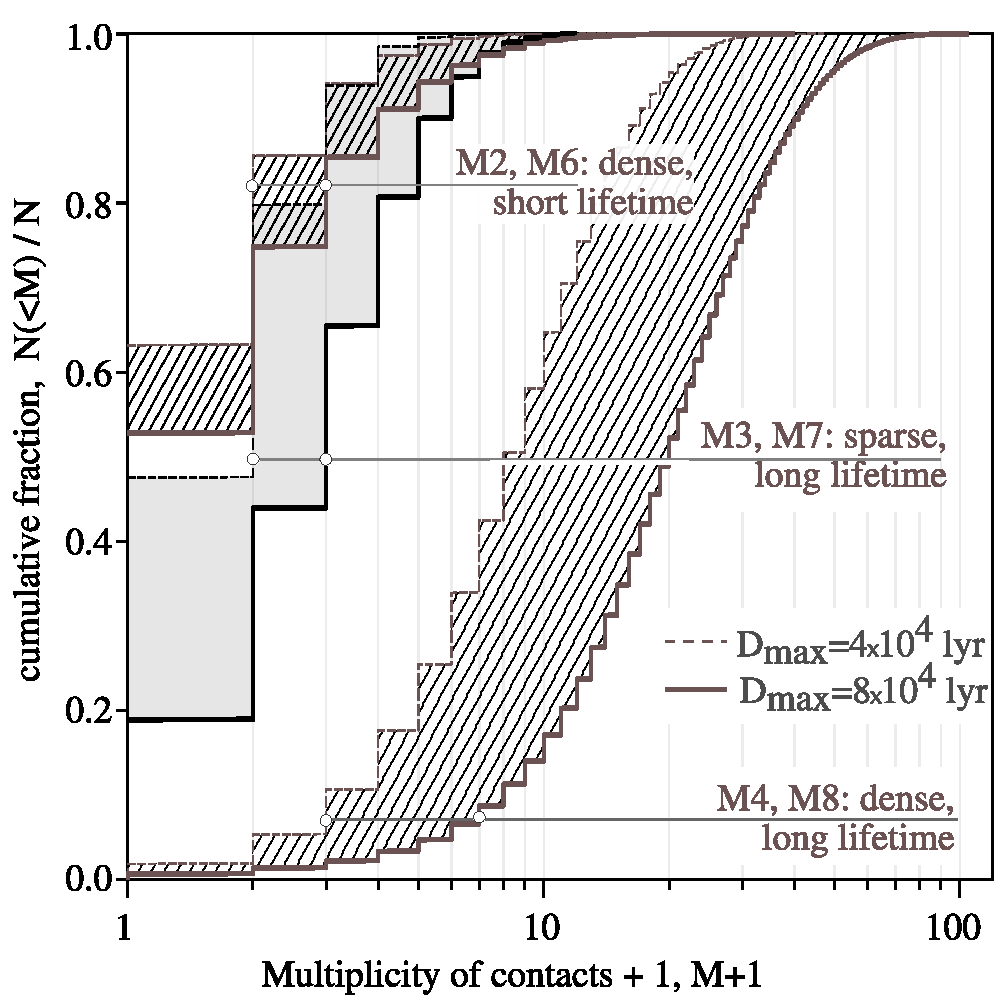
\includegraphics[width=0.5\textwidth]{F_number_of_contacts.pdf}
   \usecaption{F_number_of_contacts} \label{F_number_of_contacts}
\end{figure}
        

\subsection{Model for \cetis}
%{{{

Since the method is based on events, the first step is to define an
architecture of events, the relationships between them and how events
trigger changes on the state of the system.
%
We consider a simulated system that represents the galactic habitable
zone (GHZ).
%
On a first approach, the GHZ is a 2-dimensional annular region.
%
The adopted values for the GHZ are 20 kly and 60 kly, for the inner
and outer radius, respectively \citep{lineweaver_galactic_2004}.
% ojo, ese paper dice 7-9 kpc, o sea tiene un limite superior mucho
% mas chico...
%
This simple model does not take into account the variations in stellar
density given by the spiral structure.
%
Although there are several possible approaches, we chose to follow the
evolution of the system according to the following events:

\begin{enumerate}
   \item[(A)] Awakening: A new \ceti acquires the ability to emit
      and receive messages and starts to actively broadcast and
      lookout for messages.
   \item[(C)] Contact: A new one-way causal contact is established
      (does not require the awareness of the involved \cetis.)
   \item[(B)] Blackout: An existing causal contact is interrupted,
      with or without the occurrence of a doomsday event.
   \item[(D)] Doomsday: An old \ceti disappears, or halts its
      communication activities.
\end{enumerate}

We have chosen this nomenclature so that it can be easily remembered
from the initial A, B, C, D.
%
The \blackout is produced when one of the two \cetis halts in its
capability of emiting and receiving signals.
%
It can occur at the same time the \doomsday or before.
%
Similarly, a \ccontact can be produced at the time of the \aawakening
or later, and there can be several \contacts for the same \ceti.

                        

The system is updated each time an event is produced.
%
The time marks for each event (A and D for each \ceti and C and B for
each causal contact) are stored as a result of the simulation.
%
Also, the list of active \cetis is obtained as a function of time.
%
Some fixed variables must be set in order to carry out the simulation:
the size of the Galactic Habitable Zone, the mean lifetime of a \ceti,
$\tau_s$, the mean waiting time for the appeareance of another \ceti,
$\tau_a$, and the maximum distance a message can be detected.



The Galactic Habitable Zone is the only one of the four parameters
that is barely known, is set at fixed values of the inner and outer
radii, radial symmetry is assumed, and the with of the galactic disk is
neglected compared to the radial size.
%
The two radii are measured in light years, with the aim to maintain a
single and comprehensive unit for both space and time coordinates. 

The simulation was implemented on a python 3 code, which is publicly
available\footnote{https://github.com/mlares/simu\_contact}

%}}}
                      

%%% S E C T I O N - - - - - - - - - - - - - - - - - - - - - - -

\setlength{\tabcolsep}{10pt}
\begin{table*}
\centering
\begin{tabular}{clccc}
\hline
   \multicolumn{2}{l}{independent variables} &min&max&Nbins\\
\hline
   $\tau_{a}$ & Mean temporal separation between consecutive awakenings & 4000 y & 200000 y & 50\\ 
   $\tau_{s}$ & Mean lifetime of a \ceti                                 & 10000 y & 500000 y& 50\\ 
   D$_{max}$ & Maximum reach of a message  &  \multicolumn{3}{l}{500, 1000, 10000, 20000, 40000, 80000 lyr}  \\
\hline
   \multicolumn{4}{l}{fixed variables and assumptions} &value \\
\hline
   & statistical properties of all \cetis &equally distributed&&\\
   & Point process for the distribution in time & homogeneous &&\\
   f$_s$ & The scan of the sky & fully efficient&&1\\
   f$_p$ & panspermia or colonization &absent&&0\\
   & shape of the Galactic Habitable Zone & 2--dimensional ring &&\\
   R$_{SFC}$   & Inner radius of the GHZ     &&&20000 ly\\
   R$_{SLC}$   & Outer radius of the GHZ     &&&60000 ly\\
   t$_{max}$ & Time span of the simulation  &&&1.e6 y\\
\hline
   \multicolumn{5}{l}{discrete events}\\
\hline
   A & Awakening: a civilization starts a SETI program  &&&\\
   B & Blackout: the end of the communication channel stops &&&\\
   C & Contact: a new causal contact is produced &&&\\
   D & Doomsday: a civilization ends its communication capabilities&&&\\
\hline

\hline
\end{tabular}
\caption{Definition of independent variables and adopted values for 
   fixed parameters 
   that are part of the simulation.  Variable parameters define the
   spatial and temporal structure
   of the process and the maximum reach of the messages.}
\label{T_simu_hypotheses}
\end{table*}

 


\begin{figure*} % 2D color plot
   \centering
   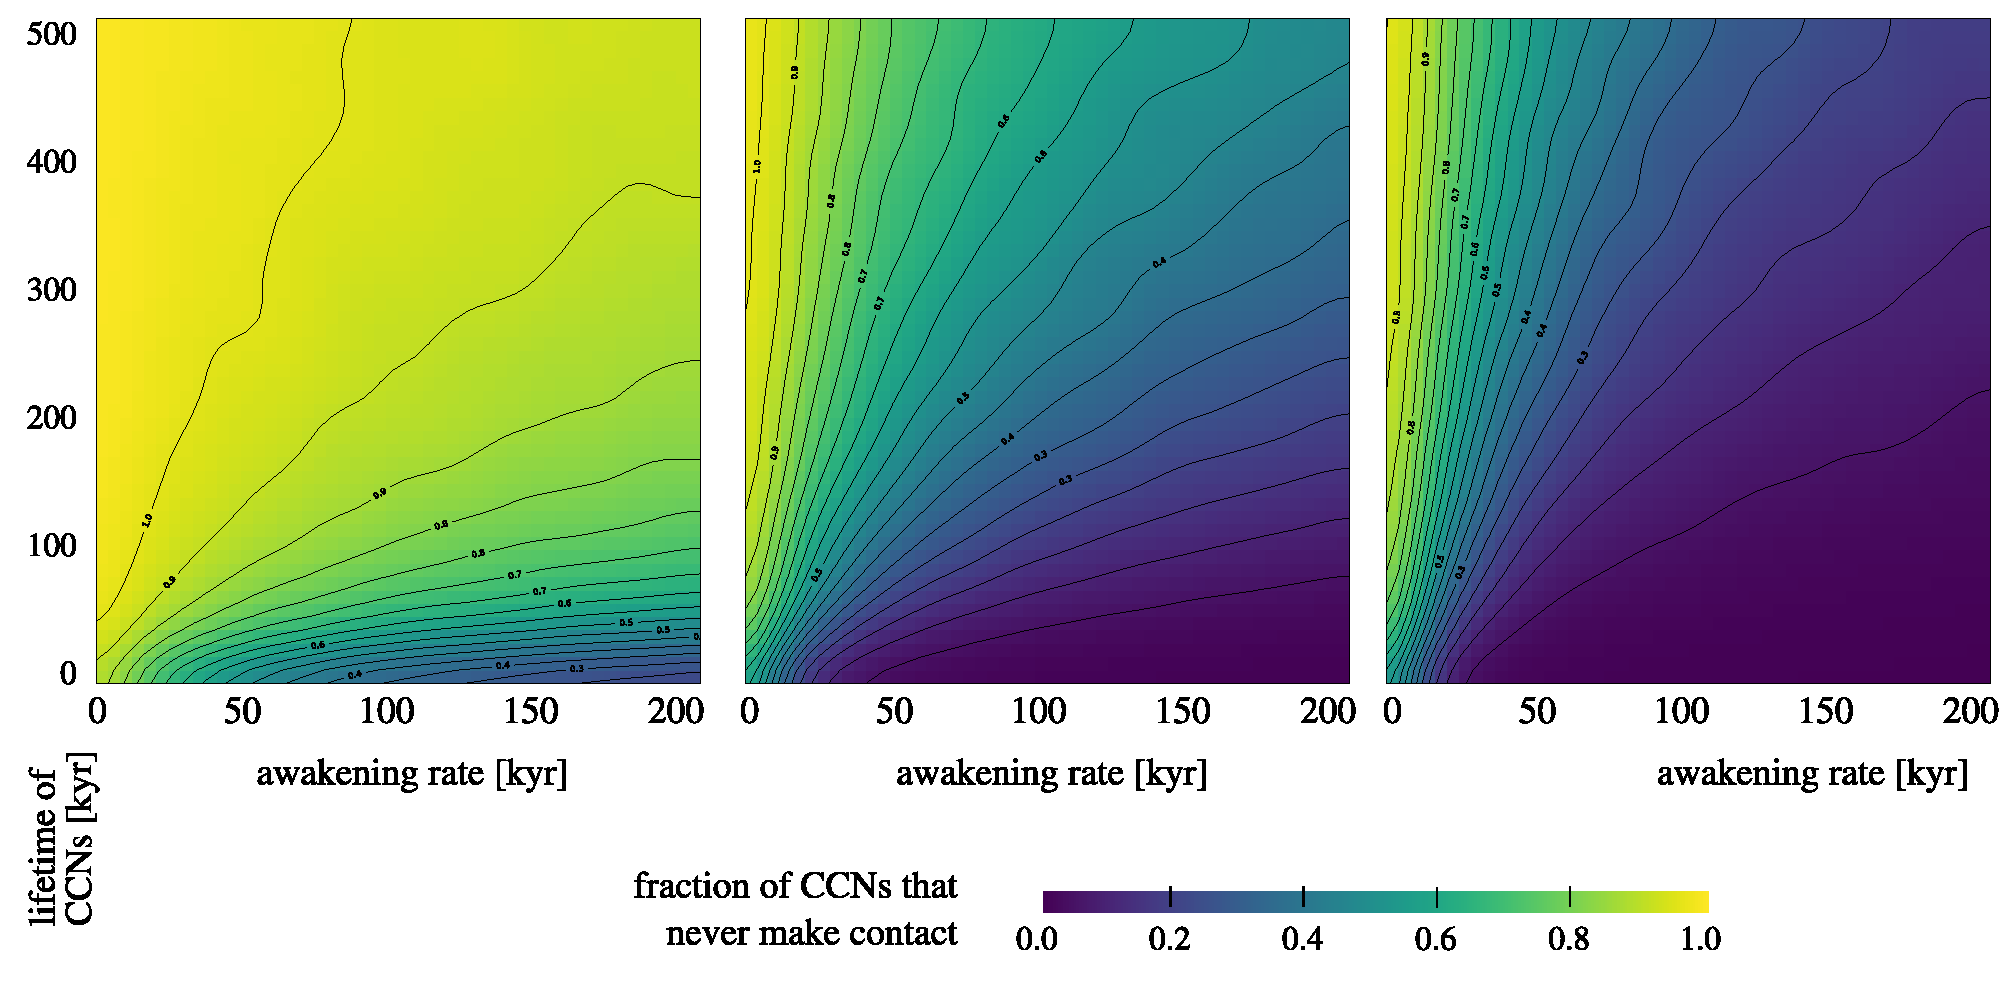
\includegraphics[width=\textwidth]{F_never_contact.pdf}
   \usecaption{F_never_contact}
   \label{F_never_contact}
\end{figure*}
 
\begin{figure*} % 2D color plot
   \centering
   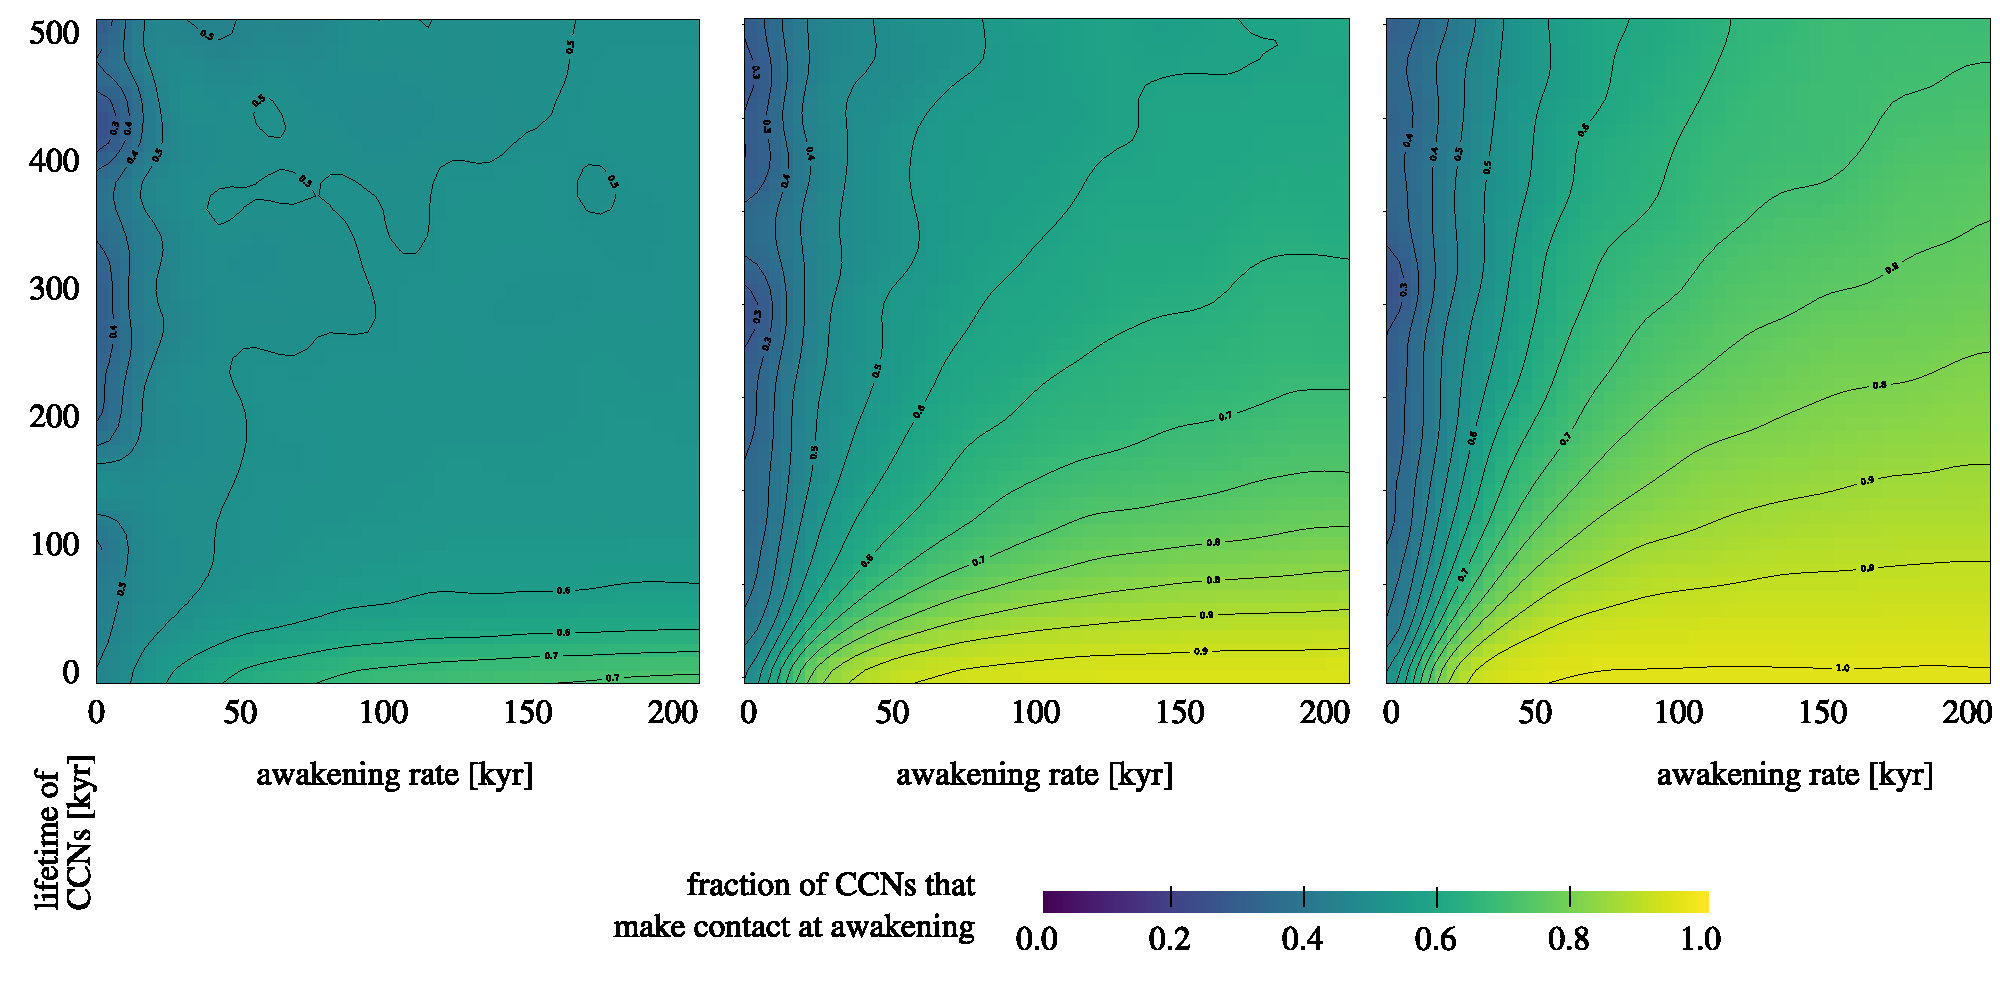
\includegraphics[width=\textwidth]{F_C_at_A.pdf}
   \usecaption{F_C_at_A}
   \label{F_C_at_A}
\end{figure*}
 
\begin{figure}
   \centering
   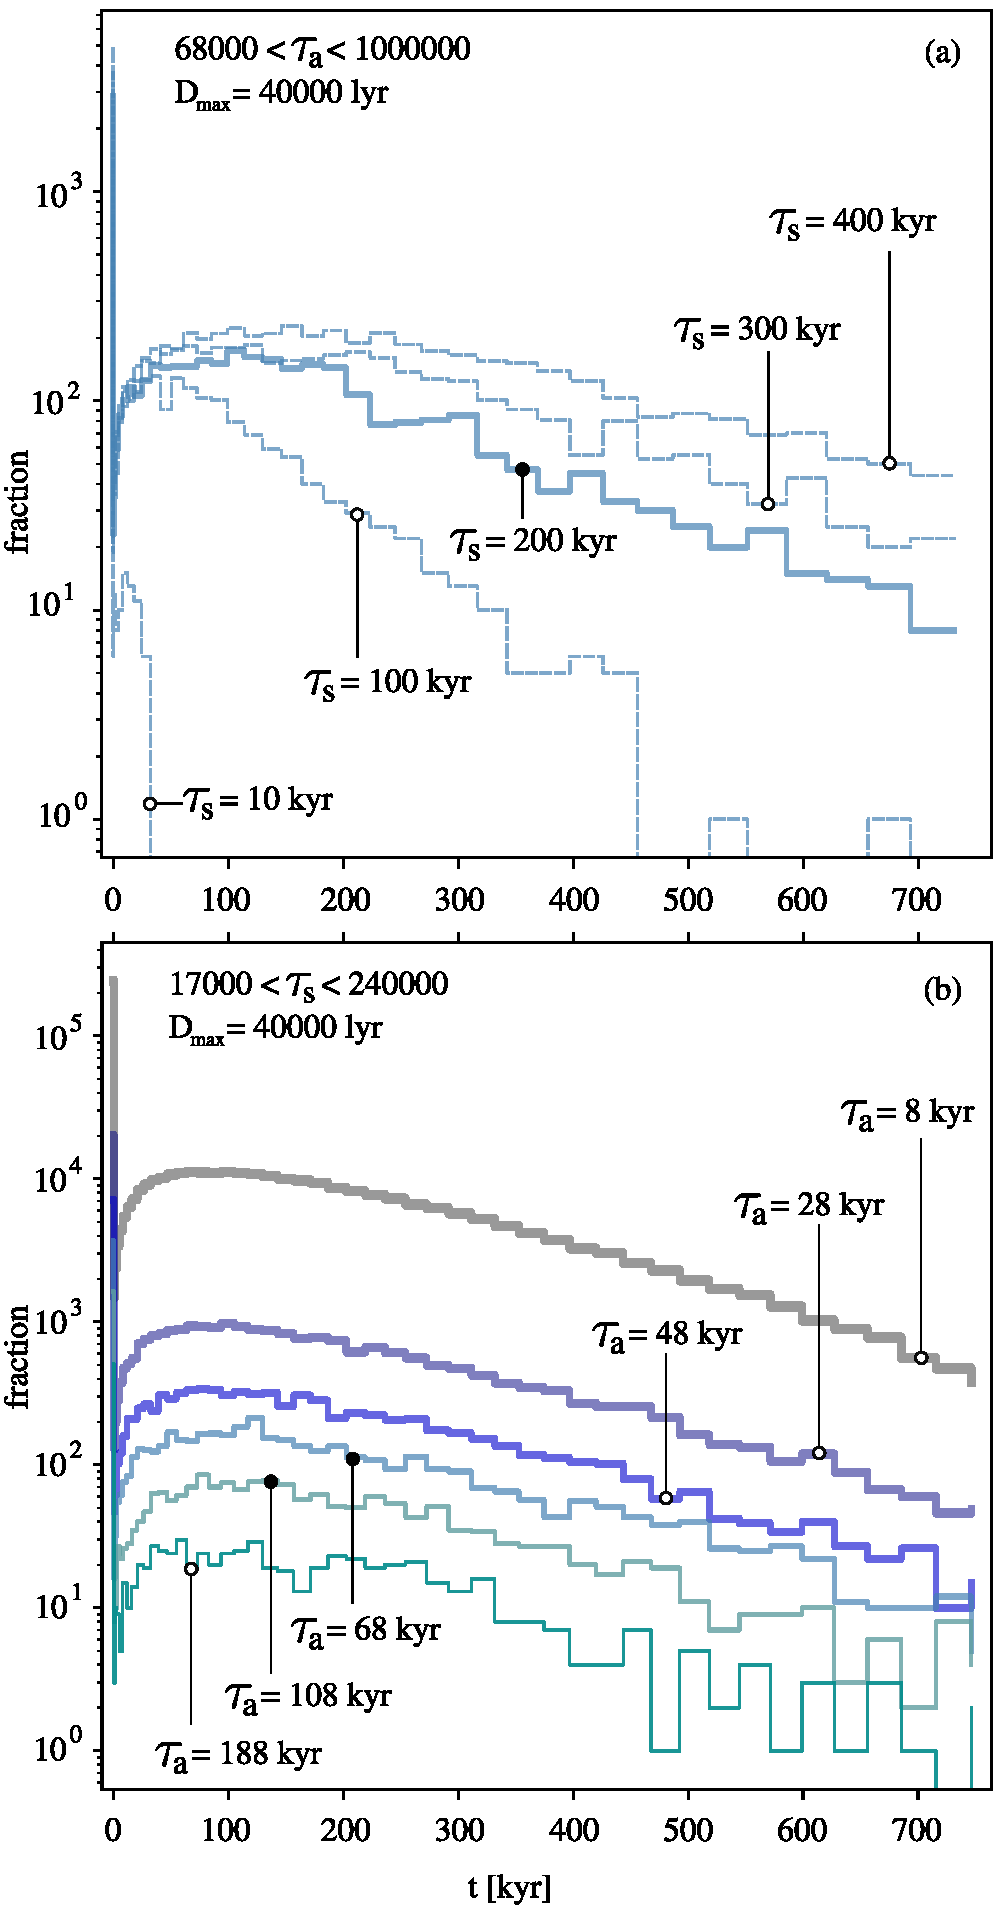
\includegraphics[width=0.5\textwidth]{F_waiting_for_1C.pdf}
   \usecaption{F_waiting_for_1C}
   \label{F_waiting_for_1C}
\end{figure}

 

%%% S E C T I O N - - - - - - - - - - - - - - - - - - - - - - -
\section{Results: exploring the parameter space}\label{S_results}
%{{{

We implemented the simulation of a regular grid of models varying over
the hypothesis space, which covers 15000 different models.
%
For each model, we simulated 50 realizations with different random
seeds, in order to perform a MonteCarlo estimation of the variance.
%
The parameters for the temporal aspects of the simulation (the mean
waiting time for the next awakening $\tau_a$ and the mean lifetime
$\tau_s$) cover the ranges 4000-200000 yr and 10000-500000 yr,
respectively, with a regular partition of 50 values for each
parameter.
%
For the D$_{max}$ parameter, we chose the values 500, 1000, 10000,
20000, 40000 and 80000 lyr.
%
This setup makes a total of 750000 simulations, each covering a time
range of one million years.
%
In Table \ref{T_simu_hypotheses} we show the set of fixed parameters
and hypotheses that define the runs of the simulations, along with the
list of variable parameters and the range of their values that have
been explored in the numerical experiments.


As a product of the simulations, several quantities can be obtained.
%
Some quantities are directly derived from the discrete events, namely,
the ID of emitting and receiving \cetis, the position in the galaxy, and
the times of each of the events that are relevant to keep track of the
number of \cetis (time of awakening and time of doomsday) and of the
number of contacts (the times of contacts and the times of blackouts).
%
We can also derive the additional quantities that represent the
properties of the \cetis, for example the total time elapsed between the
awakening and the doomsday of each \ceti.
%
The time span of a \ceti listening another or being listened by another
can also be easily derived from the results of a realization.
%
This way we can also compute the distribution in the galaxy of \cetis
that reach contact and the waiting time until the first contact or the
waiting time until the next contact.
%
Regarding the properties of the population of \cetis and its evolution,
the simulation yields the fraction of awaken time a \ceti is listening
at least another \ceti (i.e., in their causal cone), the age of
contacted \cetis at first contact, the distribution of time to wait
until next contact, the fraction of \cetis where the first contact is
given at the awakening, the distribution of the number of contacts for
each \ceti, the distribution of the number of contacts as a function of
\ceti age, the number of contacts as a function of time in the galaxy,
the rate of \cetis that succeed in contact, and the distribution of
distances between contacted \cetis.
%
Another useful derived quantity is the duration of two-way
communication channels or the fraction of contacts that admit a
response.
% 
It is also possible to analyze the relations between the distance to
\ceti vs. the time of double communication, the distance to \ceti vs. the
age of contacted \ceti, the age of a \ceti and the maximum number of
contacted \cetis before doomsday, or the lifespan of a \ceti vs. the
maximum number of contacts.
%
In addition, all these quantities can be analyzed as a function of the
simulation parameters.
%
We chose eight models that are on fairly opposed regions of the
explored parameter space, and cover short/long lifetimes, short/long
waiting times for the next \ceti to appear in the Galaxy and short/large
range reach of the signal, including all possible combinations.
%
The details of each model are summarized in the
Table~\ref{T_selected_models}.



In Fig.~\ref{F_number_of_contacts} we show the Empirical cumulative
distributions of the number contacts for \cetis in four different
samples (M5, M6, M7, M8) with long range signal reach
(D$_{max}$=10000). 
%
The lifetime is more determinant than the awakening rate in increasing
the number of contacts.
%
As expected, of the four samples, the sample M7, which corresponds to
a dense awakening in the timeline and a long lifetime, is the model
that maximizes the number of contacts, reaching a maximum of order 100
contacts for a single \ceti.
%
This is considerable larger than any model with a shorter lifetime,
which produce a number of contacts of at most the order of ten
contacts per \ceti.
%
A couple of comments are worth to mention about this plot.
%
First, it has a logarithmic scale on the x-axis, and second it is the
cumulative, not differential, empirical distribution.
 

In what follows, we focus on the analysis of the duration of contacts
(Sec.~\ref{SS_multiplicity}), the waiting time for the first contact
(Sec.~\ref{SS_waiting}) and the
variations of contact possibilities as a function of the position of
the \ceti in the Galaxy (Sec.~\ref{SS_location}).

%}}}



\subsection{Waiting time for a first contact}\label{SS_waiting}
%{{{

In this section we analyze the distribution of the waiting times for
a first contact.
%
%Such distribution can be considered to compute the probability of
%reaching a first contact within the first XX years of a SETI project,
%assuming the methods are correct and the hypotheses of the experiment.
Such distribution can be considered to compute the probability for a
random \ceti to carry out a SETI project and spend a given time until
the first contact is made. 


In the Fig.~\ref{F_waiting_for_1C} we show the fraction of the \cetis
that have made at least one contact as a function of the elapsed time
since the awakening, given that they make at least one contact on
their lifetime, for different models.
%
From a frequentist approach, the normalized cumulative counts are
related to the estimation of the probability of observing a given time
with no success.
%             
Both panels show the histograms of the waiting times for the first
contact, for all the \cetis that make at least one contact along their
lifetime.
%
We show separately the histograms for several values of $\tau_a$ and a
fixed value of $(\tau_s, D_{max})$, and for several values of $\tau_s$
and a fixed value of $(\tau_a, D_{max})$.
%
For different values of $\tau_a$, the shape of the distribution is
similar, and the main difference given by the different number of
contacts on the different models.
%
Conversely, for different values of $\tau_a$, the shape of the
distribution is similar, and the main difference given by the
different number of contacts on the different models. 
%
We show the 2D maps of the rate of \cetis that never make contact and
the rate of \cetis that make contact at the moment of the awakening,
in the Figs.~\ref{F_never_contact} and \ref{F_C_at_A}, respectively,
as a function of $\tau_s$ and $\tau_s$.
%
In the Fig.~\ref{F_waiting_for_1C} we show the histograms of the mean
waiting times for the first contact, for several models.
%
Left panel shows the histograms for several values of $\tau_a$, and
$\tau_s$ in the range 17000-24000 yr.
%
Right panel shows the histograms for several values of $\tau_s$, and
$\tau_a$ in the range 68000-100000 yr.
%
The shape of the histograms does not change when $\tau_a$ is modified,
but significantly changes when $\tau_s$ is modified.


%}}}

\subsection{Location within the Galaxy}\label{SS_location}
%{{{
    
%On the Figure~\ref{F_radial_frac} we show the fraction of \cetis that
%make zero, one, two or three contacts, as a function of the
%galactocentric distance, for model M1.  VERIFICAR!  M1?
%
For this model, the majority of \cetis do not make any contact during
all the time period in which they are active.
%
As expected, the fractions of \cetis making at least one contact
diminishes as the number of contacts rises.
%
The shape of this distribution is a result of the geometry of the GHZ.
%
In general, a closer position to the center of the Galaxy slightly
favours the possibility of a contact.
%
This would indicate that the position of the Earth is suitable for the
odds of making a contact.

%}}}



\setlength{\tabcolsep}{10pt}
\begin{table*}
\centering
\begin{tabular}{ccccc}
\hline
Model subset & D$_{max}$ & $\tau_a$ & $\tau_s$ & description  \\
\hline
M1 & 40000 & [10000, 30000]   & [10000, 50000]   &dense, short lifetime\\
M2 & 40000 & [170000, 190000] & [10000, 50000]   &sparse, short lifetime\\
M3 & 40000 & [10000, 30000]   & [400000, 440000] &dense, long lifetime \\
M4 & 40000 & [170000, 190000] & [400000, 440000] &sparse, long lifetime\\
%
M5 & 80000 & [10000, 30000]   & [10000, 50000]   &dense, short lifetime\\
M6 & 80000 & [170000, 190000] & [10000, 50000]   &sparse, short lifetime\\
M7 & 80000 & [10000, 30000]   & [400000, 440000] &dense, long lifetime \\
M8 & 80000 & [170000, 190000] & [400000, 440000] &sparse, long lifetime\\
%
\hline
\end{tabular}
\caption{Selected models to analyze the behavior of simulation outputs
   and their dependence on simulation outputs and their dependence on
   simulation parameters.}
\label{T_selected_models}
\end{table*}

 



%%% S E C T I O N - - - - - - - - - - - - - - - - - - - - - - -
\section{Discusion}\label{S_discussion}
%{{{

We have implemented a suite of simulations following a stochastic
approach, to explore the hypothesis space of a simple model that
accounts for the causal connections between communicating
civilizations on an simplified galaxy.
%
The different models can be generated with a minimal number of free
parameters and some fixed assumptions.
%
We argue that three parameters can be used to describe a variety of
situations, ranging from a Galaxy where an intelligent civilization is
very rare, to a Galaxy populated with plenty of civilizations in
causal contact.
%
We explored the consecuences of different models using mensurable
quantities, that arise as by-products of the simulations.
%
With this approach, we can estimate several quantities as a function
of the parameters on the hypothesis space.
%
For instance, it is possible to estimate the timescale for an
uninterrupted SETI effort to reach success, in terms of different
model parameters that reflect different, so far unknown, scenarios for
the spread of intelligent life on the galaxy.


Although the simulations use a number of speculative assumptions, we
argue that the degree of knowledge about the origin and persistence of
life in the Galaxy does not worth the implementation of more detailed
or sophisticated models.
%
Instead, we take advantadge of the simplicity of the model to explore
the hypothesis space, i.e., the three--dimensional parameter space of
the parametric model, in order to gain insight on the consecuences of
different scenarios for the search of intelligent life.
%
Our analysis is not centered in obtaining the odds for the Earth
making contact with another extraterrestrial civilization, but in
obtaining a statistical, parameter dependent description of the
communication system consisting of a group of broadcasting
civilizations which arise sparsely both in time and space in the
Galaxy.



Under the hypotheses of our experiments, we conclude that a causal
contact is extremely unlikely unless the Galaxy is heavily populated
by intelligent civilizations.
%
Even so, we must consider that in order to stablish a contact between
any two entities, a minimum degree of compatibility must be
accomplished without any previous agreement, making the posibility of
a contact with a message that could be deciphered highly rare.



Taking into account the caveat mentioned previously about the
trade--off between the simplicity and complexity of the experiment,
future work can be performed following this framework in order to
explore possible implications of the results for more detailed
configurations.
%
For example, the communication method (isotropic, colimated,
serendipitous) can affect the observables.
%
Since we analyze the causal contacts, effective contacts depend on the
efficiency of both the emitter and the receiver.
%
A correction by coverage ratio in the detection and by a targetting
ratio in the emission could be easily implemented in the simulation,
although the effect would be to reduce the probability of contact by
an efficiency ratio.
%
Thus, such implementation is not really necessary, since the values of
probabilities could modified by a constant correction factor equal to
the combined emission/reception efficiency
\citep{smith_broadcasting_2009, anchordoqui_upper_2019,
forgan_collimated_2014}.
%
If we consider a statistical distribution for this factor, then the
results could change, and this could be studied with the DE approach.
%
Also the nature of the message carrier, electromagnetic or another.
%
It is also possible to explore the effects of alignments or the use of
stars as sources or amplifiers.
%
%energetic markers Spiritual markers
%
As a future work, we will explore several improvements to the
simulation, and analyze the impact on the final results of these
changes.
%
They include a spatial distribution that actually resembles the shape
of the Galaxy, different distribution functions for the mean lifetime
of MPLs and different efficiencies for the sphere of the causal region
of each MPL, resembling different searching strategies
\citep{hippke_interstellar_2017}.


Possible hypothesis improvements are:

\begin{itemize}
   \item D$_{max}$ is different for different MPLs.  For example a power
      law where powerfull emmisions are rare and weak emssions are
      common.
   \item The probability of the rising of a new MPL vary within the GHZ.
   \item Correction by coverage ratio in the detection and by
      targetting ratio in the emission.
   \item Explore the role of the message
      contents, influence on the lifespan of a MPL that receives a
      message, mean lifespan of a MPL that emits a message.
\end{itemize} 

 
%}}}


\ack[Acknowledgement]{
%
This work was partially supported by the Consejo Nacional de
Investigaciones Cient\'{\i}ficas y T\'ecnicas (CONICET, Argentina),
the Secretar\'{\i}a de Ciencia y Tecnolog\'{\i}a, Universidad Nacional
de C\'ordoba, Argentina, and the Universidad Cat\'olica de C\'ordoba,
Argentina.
%
This research has made use of NASA's Astrophysics Data System.
%
Plots and simulations were made with software developed by the authors
using R and python languajes. Plots were postprocessed with inkscape.
%
}


\ack[Disclosure statement]{
%
No competing financial interests exist.
%
}


\bibliographystyle{mn2e}
\setlength{\bibsep}{0.0pt}

\bibliography{biblio_seti}

\end{document}
